\title{DBScan}
\label{chp:dbscan}
\author{Lina Yao}
\institute{School of Computer Science and Engineering, University of New South Wales, Australia}
\maketitle


%\section{Overview}
The Density Based Spatial Clustering of Applications with Noise (DBSCAN) 
algorithm was first proposed in 1996 by \cite{ester1996density}. It has been 
proven to have promising performance in various applications, and it received 
the SIGKDD test-of-time award in 2014.  DBSCAN is a unsupervised machine leanring and density-based clustering method. 
It aims for identifying high-density regions in data space and treating them as 
clusters, separated by regions of low point density. Let's starting by an 
illustrative example for better understanding the density. Taking a look at Figure~\ref{fig:example}, there 3 sets of sample points. Intuitively, we can identify thoese clusters of points and unclusterred outliers straightforwardly, no matter how those sample points are distributed or in what shapes. By instinct, we natually observe and recognize the density differences within those areas and consider each cluster of points have higher denseness. While the rest points of considerably lower densities are regarded as noises and belongs to no cluster~\cite{ester1996density}. Based on a set of points in this 
example, DBSCAN groups together points that are close to each other based on an 
arbitrary distance measurement in different application domains 
(e.g., Euclidean distance) and a minimum number of points that is a threshold to 
distinguish the outliers in the lower density regions. 


\begin{figure}[tbp]
	\centering
	\label{fig:example}
	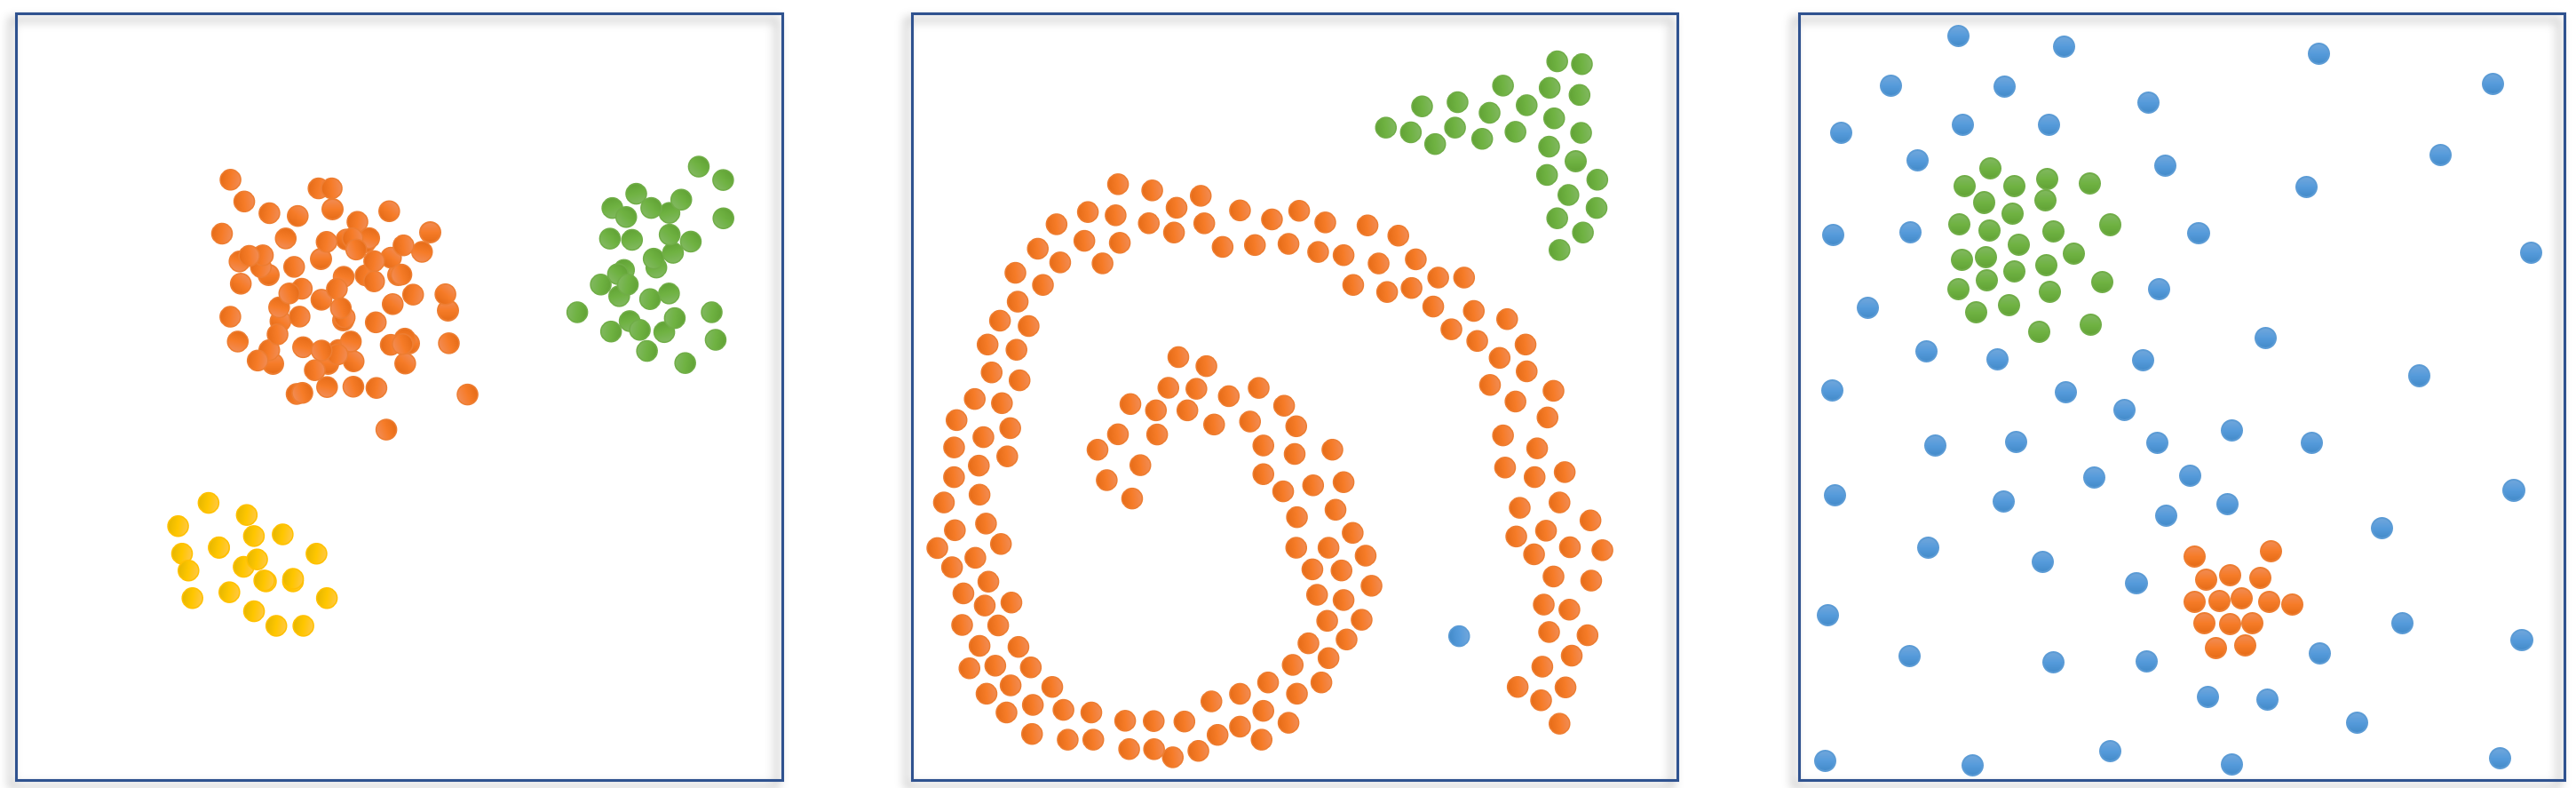
\includegraphics[width=\textwidth]{"Part 3 - Learning Systems/Unsupervised Learning/DBScan/figures/example_density.png"}
	\caption{Samples for density illustration. Different colors represent different clusters of points}
\end{figure}


\section{The Algorithm}

Suppose we have a set of data points \[\mathcal{X} = 
\{\mathbf{x}^{(1)},\mathbf{x}^{(2)},\cdots,\mathbf{x}^{(N)}\}\]
\noindent where $\mathbf{x}^{(i)} \in \mathcal{X}$ are drawn i.i.d. 
(independently and identically distributed).  The core idea of DBSCAN is to 
estimate the density for each data point $x^{i}$ as a minimal number of 
$MinPts$ of points that lie inside a radius $\epsilon$ around $x^{i}$. 
% Points are considered directly connected if the distance between them is no greater than $\epsilon$. 
Points with distances to each other no greater than a pre-defined threshold $\epsilon$ can be deemed connected and within the same cluster.
As such, DBSCAN has two key parameters. 

\begin{itemize}
	\item{$\epsilon$} is a positive real value. It is defined using a distance 
	function and specifies the neighborhoods. Two points are considered to be 
	neighbors if the distance between them are less than or equal to 
	$\epsilon$, i.e., $dist(\mathbf{x}^{(i)} - \mathbf{x}^{(j)}) \leq \epsilon$. The data 
	points within a radius of $\epsilon$ from a given point $\mathbf{x}^{(i)}$, 
	form its $\epsilon$-Neighborhood denoted as 
	$\mathit{N_{\epsilon}(\mathbf{x}^{(i)}):\{\mathbf{x}^{(i)}| 
	dist(\mathbf{x}^{(i)}, \mathbf{x}^{(j)})\leq \epsilon\}}$
	
	\item{$MinPts$} is a small positive constant integer, that specifies the 
	minimum number of data points to define a cluster.	
\end{itemize}

If the neighborhood $N_{\epsilon}(\mathbf{x}^{(i)})$ contains a number of points equals to or more than $MinPts$, it's called high density, otherwise it is low density. For example, 
if we set $MinPts = 4$ in Figure \ref{fig:relation}, 
$\epsilon$-Neighborhood of point $A$ is a high density area since it has 5 
points including $A$ itself in its surrounding neighbourhood, which is more 
than $MinPts = 4$, while $\epsilon$-Neighborhood of point $C$ is low density 
area since its only has 2 points including $C$ itself. Up to this point, we have defined two key parameters, $MinPts$ indicates the  density and $\epsilon$ indicates the radius of $\epsilon$-Neighbourhood, and  gained the 
basic understandings of measuring the density. The points in a given dataset 
are then classified into the following categories. 


\begin{figure}[tbp]
	\centering
	\includegraphics[width=\textwidth]{"Part 3 - Learning Systems/Unsupervised Learning/DBScan/figures/illustration of 
		DBSCAN.png"}
	\caption{In this example, the minPts parameter is 4, and the $\epsilon$ 
		radius is indicated by the circles. Red point is a outlier point, which 
		is 
		not density reachable. Green points are a core point, and pale blue 
		points 
		are border points. Double arrows indicate direct density reachability, 
		which is symmetric. Arrows connecting the border points B and C 
		indicate 
		density connected, while both are density reachable from the A. The 
		density 
		connectivity is asymetric. N is not connected indicating not density 
		reachable, and thus considered to be a outlier point/noise. Figure adapted from 
		Schubert et al. 
		\cite{schubert2017dbscan}
	}
	\label{fig:relation}
\end{figure}



\begin{itemize}


\item\textit{Core point}. A core point has a $\epsilon$-neighbourhood with more than $MinPts$ data points (including the given point itself); 

\item\textit{Border point}. A border point locates in the neighborhood of certain core point, but itself has a number of points less than $MinPts$ within its $\epsilon$-Neighbourhood;


\item\textit{Outlier}. A point that is neither a core point nor a 
border point. 
	
\end{itemize}

As recalled, the intuition of DBSCAN is to find the regions in a data space 
which have higher density, separated by regions of lower density. In other 
words, to group each data point in a cluster which contains at least $MinPts$ 
number of points in the $\epsilon$-neighbourhood of this point. If this point is a core point, and then it forms a cluster along with all data points including core points and border points that are reachable from it. $\epsilon$-neighbourhood of certain border point usually has fewer points than the 
$\epsilon$-neighbourhood of points located within its cluster. A very small 
$MinPts$ is necessary to be set to group all the points belonging to a same 
cluster. However, it would also cause a problem in distinguishing points from 
the data noise/outlier. To tackle this issue, DBSCAN requires that given every 
point $\mathbf{x}^{(i)}$ in a cluster where there is a point $\mathbf{x}^{(j)}$ so 
that $\mathbf{x}^{(i)}$ is within $\epsilon$-neighbourhood of $\mathbf{x}^{(j)}$ 
and its neighbourhood has more than $MinPts$ number of points. To achieve this, 
the different levels of density reachability are defined \cite{ester1996density}


\begin{itemize}
\item \textit{Directly density-reachable}.  
%A point $\mathbf{x}^{i}$ is 
%directly 
%density-reachable 
%from $\mathbf{x}^{j}$ if $\mathbf{x}^{i}$ is a core point and 
%$\mathbf{x}^{j}$ is in the neighborhood of $\mathbf{x}^{i}$. 
Point $\mathbf{x}^{(i)}$ 
is directly density-reachable from a point $\mathbf{x}^{(j)}$ wrt. $\epsilon$ and 
$MinPts$ if $\mathbf{x}^{(j)} 
\in  \mathit{N_{\epsilon}(\mathbf{x}^{(i)}):\{\mathbf{x}^{(i)}| 
	dist(\mathbf{x}^{(i)}, \mathbf{x}^{(j)})\leq \epsilon\}}$ and 
$|N_{\epsilon}(\mathbf{x}^{(j)})| \geq MinPts$. Obviously, directly 
density-reachable is symmetric for core point pairs. For instance, core points A, A' and A'' are directly reachable in Figure~\ref{fig:relation}. 
% This relation is not symmetric if one core point and one border point are involved. 
Such symmetric relationship cannot be established for a core point and a border point. 

\item \textit{Density-reachable.} A point $\mathbf{x}^{(i)}$ is density reachable from a point $\mathbf{x}^{(j)}$ wrt. 
$\epsilon$ and $MinPts$  if there is a chain of points $\mathbf{x}^{(i)}, \mathbf{x}^{(i+1)}, ..., \mathbf{x}^{(j)}$ where from $i$ to $j$, all points satisfy that $\mathbf{x}^{(i+1)}$ is directly density-reachable from $\mathbf{x}^{(i)}$. For instance, point B is density-reachable from A, while A is not density-reachable from B in Figure~\ref{fig:relation}. Density-reachability is a canonical extension of direct density-reachability. This relation is transitive, yet not symmetric. Two 
border points within the same cluster may be not density reachable from each other because the core point condition might not hold for both of them. However, there must be a core point in a cluster from which both border points of this cluster are density-reachable. Therefore, the following notion of density-connectivity is introduced to cover this relation of border points.

\item \textit{Density-connectivity.}  A point $\mathbf{x}^{(i)}$ is density connected to a point $\mathbf{x}^{(j)}$ wrt. $\epsilon$ and $MinPts$ if there is a point $\mathbf{x}^{(k)}$ such that both, $\mathbf{x}^{(i)}$ and $\mathbf{x}^{(j)}$ are 
density-reachable from $\mathbf{x}^{(k)}$ wrt. $\epsilon$ and $MinPts$. Density-connectivity is a symmetric relation. For instance, border points B and C become density-connected in Figure~\ref{fig:relation} via core points A, A' or other green core points. 
\end{itemize}

\begin{algorithm}[ht!]
    \label{algo}
    \CommentSty{\color{blue}}
    \SetAlgoLined\DontPrintSemicolon
    \SetKwFunction{DBSCAN}{DBSCAN}
    \SetKwProg{beginAlgorithm}{Algorithm}{}{}
    \beginAlgorithm{\DBSCAN{}}{
	    \KwIn{$\mathcal{X} = 
	    	\{\mathbf{x}^{(1)},\mathbf{x}^{(2)},\cdots,\mathbf{x}^{(N)}\} \in 
	    	\mathbb{R}^{d}$   \tcp*{dataset}}
	    \KwIn{$\epsilon$   \tcp*{radius distance of neighbour}}
	    \KwIn{$MinPts$ \tcp*{minimal size of a cluster}}
	    \nl $C \gets 0$   \tcp*{start with an empty cluster}
	    \ForEach{unvisited point $\mathbf{x}$ in $\mathcal{X}$}{ 
			\nl mark $\mathbf{x}$ as $Visited$ \;
			\nl $N_{\epsilon}(\mathbf{x})$ $\gets$ regionQuery($\mathbf{x}$, $\epsilon$)  \tcp*{finding initial neighbourpoints of $\mathbf{x}$}
			\uIf{$|N_{\epsilon}(\mathbf{x})|$ $<$ $MinPts$\tcp*{size of neighbourpoints of $\mathbf{x}$}} {
				\nl mark $\mathbf{x}$ as $NOISE$ \;
			}
			\uElse{
				\nl $C\gets C+1$  \tcp*{start a new cluster}\;
				\nl expandCluster($\mathbf{x}$, NeighborPoints, C, $\epsilon$, $MinPts$) \;
			}
	    } 
	}{}
    
    \setcounter{AlgoLine}{0}
    \SetKwFunction{expandCluster}{expandCluster}
    \SetKwProg{beginProc}{Procedure}{}{}
    \beginProc{\expandCluster{}}{
	    \KwIn{$\mathbf{x}$ \tcp*{current points}}
	    \KwIn{$\mathbf{x'} \in N_{\epsilon}(\mathbf{x})$  \tcp*{neighbour points of current points $\mathbf{x}$}}
	    \KwIn{$C$ \tcp*{current cluster}}
	    \KwIn{$\epsilon$}
	    \KwIn{$MinPts$}
	    \nl add $\mathbf{x}$ to cluster $C$\;
	    \ForEach{point $\mathbf{x}'$ in $N_{\epsilon}(\mathbf{x})$}{
	    	\If{$\mathbf{x'}$ is not $visited$}{
		    	\nl mark $\mathbf{x}'$  as $visited$\;
		    	\nl $N_{\epsilon}(\mathbf{x'})$$\gets$ regionQuery($\mathbf{x}'$ , $\epsilon$)\;
		    	\If{$|N_{\epsilon}(\mathbf{x'})|$ $\geq$ $MinPts$}{
		    		\nl $N_{\epsilon}(\mathbf{x}) = N_{\epsilon}(\mathbf{x})$ $\cup$ $N_{\epsilon}(\mathbf{x'})$ \;
		    	}
	    	}
	    	\If{$\mathbf{x'}$ is not a member of any cluster}{
	    		\nl add $\mathbf{x'}$ to cluster $C$
	    	}
	    }
	    \nl \KwRet\;
    }
    
    \setcounter{AlgoLine}{0}
    \SetKwFunction{regionQuery}{regionQuery}
    \beginProc{\regionQuery{}}{
	    \KwIn{$\mathbf{x}$ \tcp*{current point}}
	    \KwIn{$\epsilon$ represent min distance of neighbour}
	    \nl \KwRet all points within $\epsilon$ distance of $\mathbf{x}$\;
    }
    \caption{DBSCAN}
\end{algorithm}

Now, we have a formal notion of density. A cluster $C$ is defined to be a set of density-connected points wrt $\epsilon$ and $MinPts$, which is non-empty and satisfying the following two properties (i) Maximality: for any data point $\mathbf{x}^{(i)} \in C$ and $\mathbf{x}^{(j)}$ is density-reachable it wrt $\epsilon$ and $MinPts$, then $\mathbf{x}^{(j)} \in C$; (ii) any of two points in this cluster are density-connected. A toy 
example in Figure~\ref{fig:relation} explains the how it progresses. All 
neighbors within the $\epsilon$-neighbourhood of a core point $A$
are considered to be part of the same cluster due to they are direct 
density reachable to $A$. If any of these points in its 
$\epsilon$-neighbourhood is again a core point like 
$A'$ and $A''$, and their neighborhoods are transitively included (called 
density reachable) into the same cluster. The border points (like point $B$) in 
the same set are density connected. As the progress continues, point $B$ will 
be maximally density connected with another border point $C$ via a chain. 
Relatively, points which are not density reachable from any core point are 
considered noise and do not belong to any cluster like the red point $N$. The 
cluster is complete as it becomes surrounded by border points and there are no 
more points within $\epsilon$-neighbourhoods. A new random point will be 
selected and repeat the same process to identify the next cluster. 


The Pseduo code of DBSCAN is 
shown in Algorithm~\ref{algo}. It is noted that the RegionQuery($\cdot$) function is called for each point, which most significantly contributes to the runtime complexity of DBSCAN. The overall runtime complexity is $\mathcal{O}(n \cdot RegionQuery(\cdot))$. If this function is implemented in the most naive way, the runtime complexity of DBSCAN would be $\mathcal{O}(n^{2})$, which is the worst case. Many advanced techniques are proposed to speed up the region query, such as R-tree, KD-tree etc~\cite{schubert2017dbscan}. It is commonly recognized that the average runtime complexity of DBSCAN is $\mathcal{O}(n \cdot \log n)$.

\section{An Example of DBSCAN}

Clustering has been widely used in a variety of real-world applications like market analysis, social network analysis, segmentation and object detection. In this chapter, we demonstrate how DBSCAN can be used for object segmentation task on a RGB+Depth scene dataset, SUN RGB-D, which is a RGB-D scene understanding benchmark suite. The main objective of the clustering method is to classify the pixels into homogeneous clusters (i.e., objects) that hold on maximum similarity within the clusters while reaching the minimum dissimilarity cross the clusters. 


This SUN RGB-D dataset contains 10,000 RGB-D images. It is densely annotated and includes 146,617 2D polygons and 58,657 3D bounding boxes with accurate object orientations, as well as a 3D room layout and category for scenes.
with accurate annotations of 146,617 2D polygons, 58,657 3D bounding boxes and object orientations. A 3D room layout where the images are captured and scenario categories for the images are also available. 
The detailed description and download information can be found from here 
\footnote{\url{http://rgbd.cs.princeton.edu/}}. We use the scikit-learn 
\footnote{\url{https://scikit-learn.org/stable/modules/generated/sklearn.cluster.DBSCAN.html}}
to implement. Figure \ref{fig:scene} shows the results. We can clearly observe 
that DBSCAN can accurately segment the different shapes of furniture. 
%The 
%source code regarding this example can be found as follows.
\begin{figure}[h!]
	\label{fig:scene}
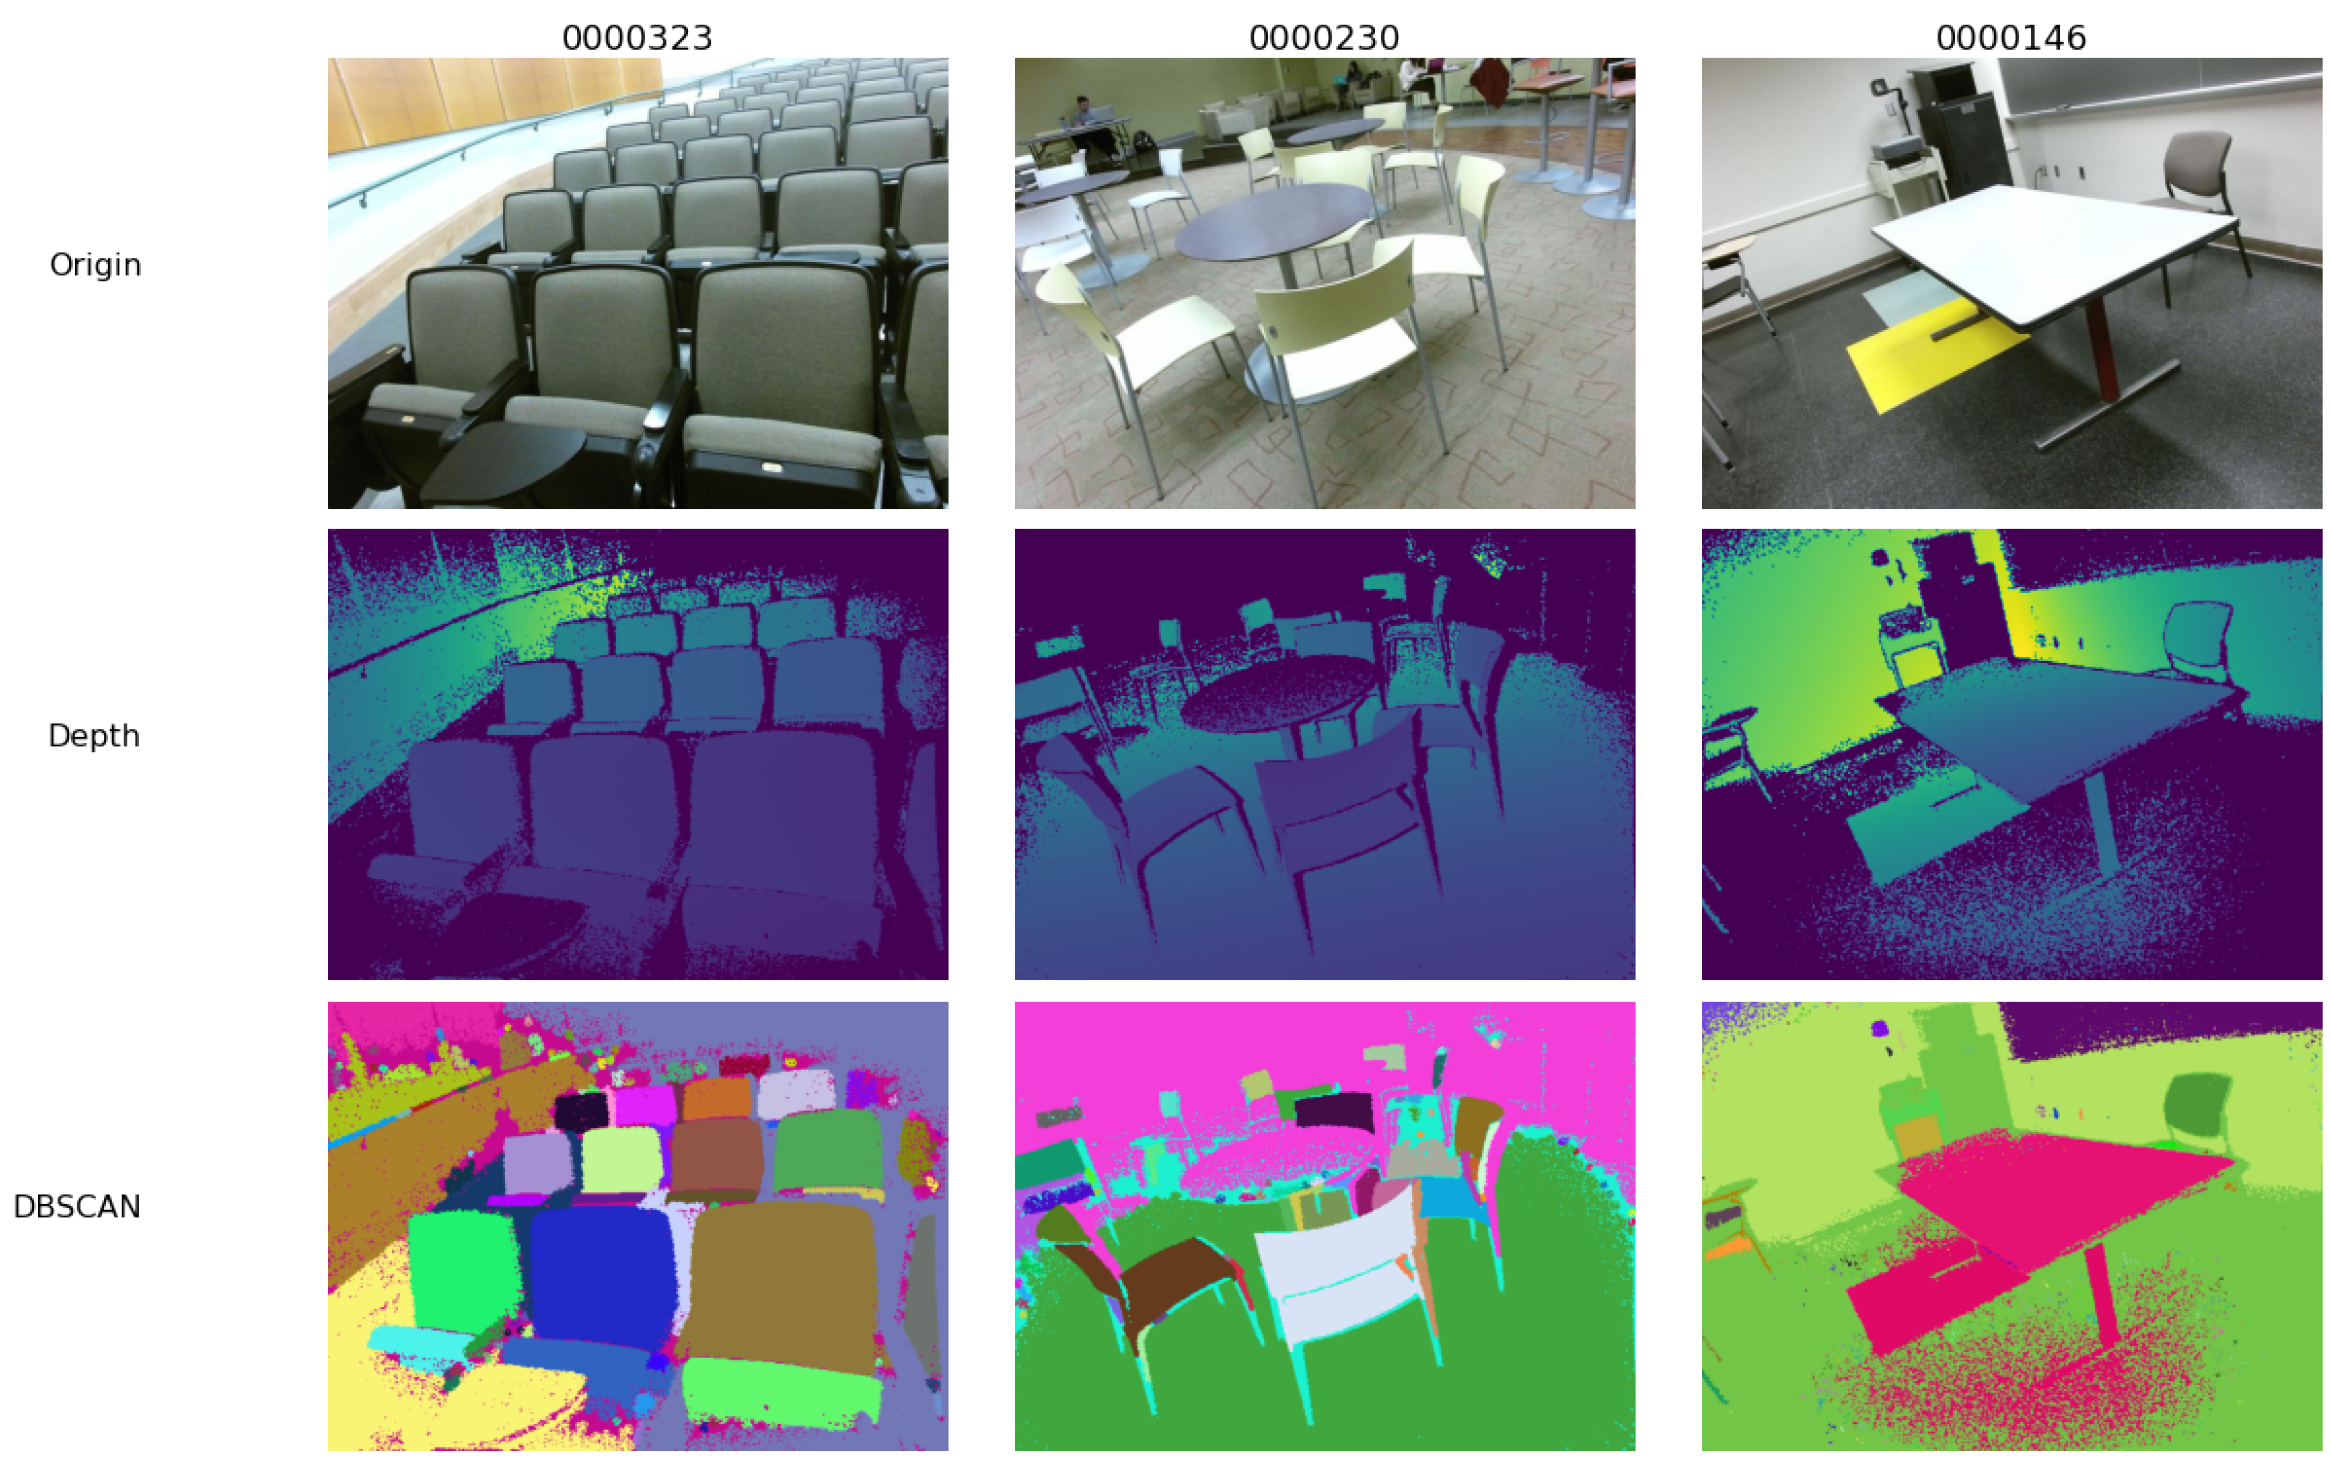
\includegraphics[width=\textwidth]{"Part 3 - Learning Systems/Unsupervised Learning/DBScan/figures/segment.png"}
\caption{Object detection using DBSCAN. The first row shows the original 
images, the second row shows the corresponding depth images, and the last row 
shows the detection results using DBSCAN.}
\end{figure}

\section{Determine $\epsilon$ and $MinPts$}

DBSCAN has 2 key parameters $\epsilon$ and $MinPts$, which can be critical to its performance. It requires joint tuning 
these two parameters to find 
the optimal combination to ensure the clustering performance. In general, 
there is no common practice to determine 
$MinPts$. It depends on domain knowledge and understanding of the given datasets. 
A low $MinPts$ means it will build more clusters from noise. In many cases, the 
domain knowledge is generally unknown especially considering that data is usually normalized 
before further processing. Ester et. al 
\cite{ester1996density} propose to use the sorted $k$-distance graph to assist with 
deciding $MinPts$. $k$-dist graph plots the average distance between each point and its $k$-nearest neighbours in ascending order, where $k=MinPts$. In their case, experiments indicate that with a  $k > 4$,  $k$-dist graphs introduce substantially more computational costs while contributing no significantly better results than the 4-dist graph.
Therefore, $MinPts = 4$ was recommended for their 2-dimensional data. It is noted that this setting may not be applicable to other datasets. 


More heuristics for $MinPts$ are proposed, 
for example, $MinPts$ can also be set as $MinPts = 
\dfrac{1}{n}\sum_{i=1}^{n}|N_{\epsilon}(\mathbf{x}^{(i)})|$, where 
$|N_{\epsilon}(\mathbf{x}^{(i)})|$ is the number of points in 
$\epsilon$-neighbourhood of given data point $\mathbf{x}^{(i)}$ and $n$ is the 
total number of data points in the dataset
\cite{sawant2014adaptive}. Another way for choosing $MinPts$ is to derive it 
from the number of dimensions $d$ of data set by taking $MinPts = 2 * d - 1$ 
\cite{sander1998density}. 

\begin{figure}
	\centering
	\label{fig:para}
	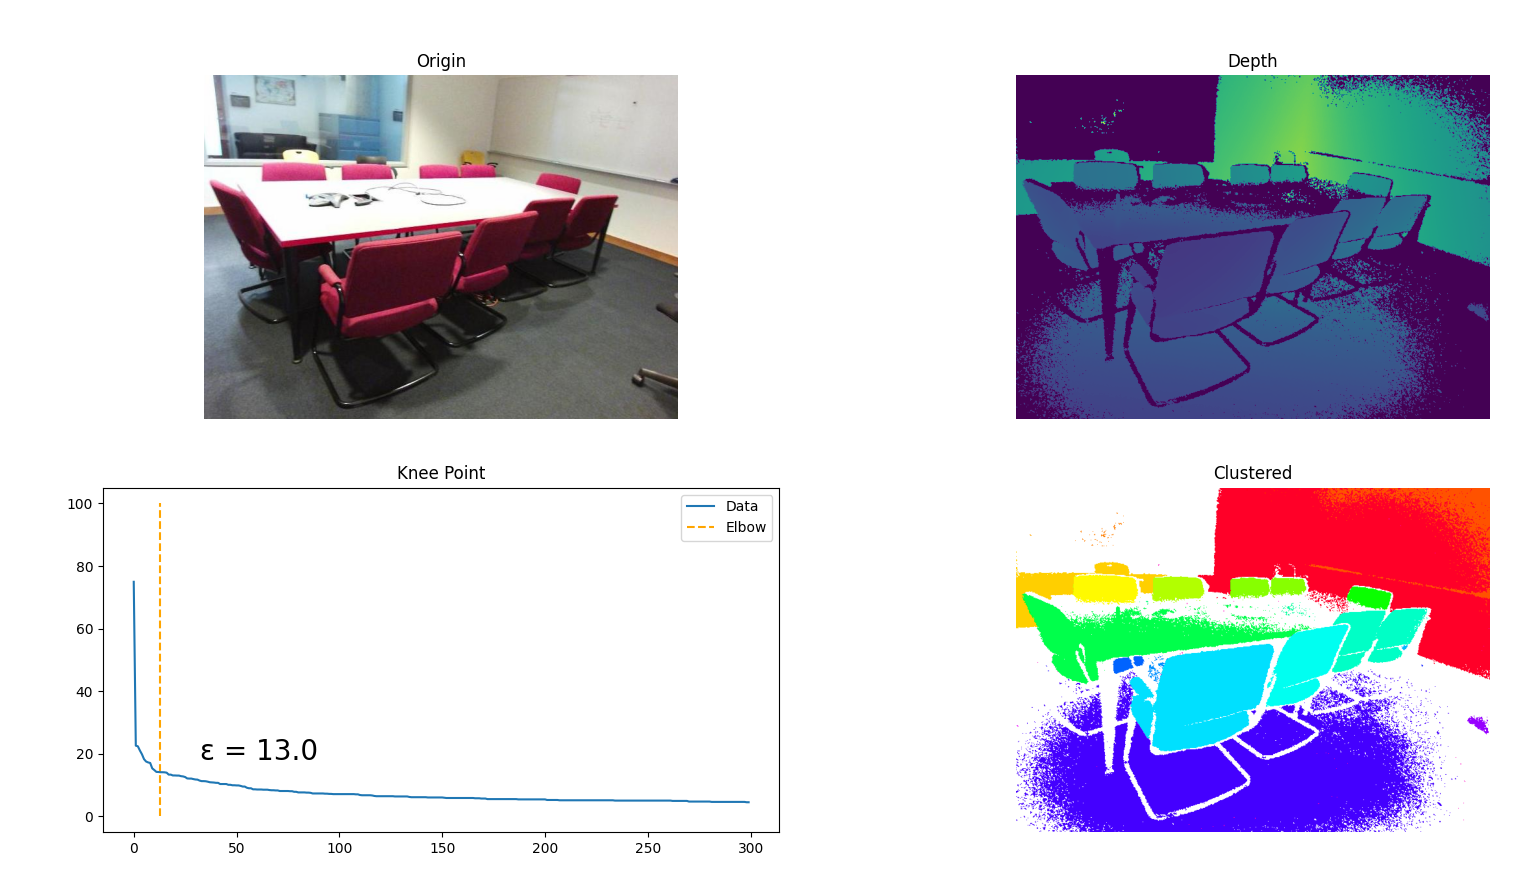
\includegraphics[width=\textwidth]{"Part 3 - Learning Systems/Unsupervised Learning/DBScan/figures/para.png"}
	\caption{An illustrative example is finding optimal $\epsilon$ given $k = 
	4$; the knee point corresponds to $\epsilon = 13.0$. The clustering result 
	shows the good performance with these two parameters.}
\end{figure}


In general, $\epsilon$ should be chosen as small as possible. However, if 
$\epsilon$ is too small, many points may be considered as outliers because a considerable amount of points may be discarded as outliers due to the very small neighborhoods, which results in many points not becoming core points or border points. While, a large value for $\epsilon$ may produce rather huge clusters with too many points inside.
In the original DBSCAN paper 
\cite{ester1996density}, an interactive approach is offered to detemine the 
optimal 
$\epsilon$.  The basic process is to first calculate the average of the 
distances of every point to its $k$ nearest neighbors, where $k = MinPts$, and 
the computed $k$-distances are plotted in a descending order. The knee point 
formed by the plot indicates a threshold where a sharp change occurs along this 
$k$-distance curve. The value of knee point is treated as the optimal 
$\epsilon$. The Figure~\ref{fig:para} shows an example of determining the 
$\epsilon$ using $k$-distance plot. 



\section{Discussion}

DBSCAN can work on discovery of clusters with arbitrary shape of datasets and 
the number of clusters that does not need to be predefined. It has good noise 
resistance and can handle noisy dataset well. The desirable range of data noise 
ratio for DBSCAN to tolerate well is between 1\% to 30\%
\cite{schubert2017dbscan}. 


\begin{figure}
	\centering
	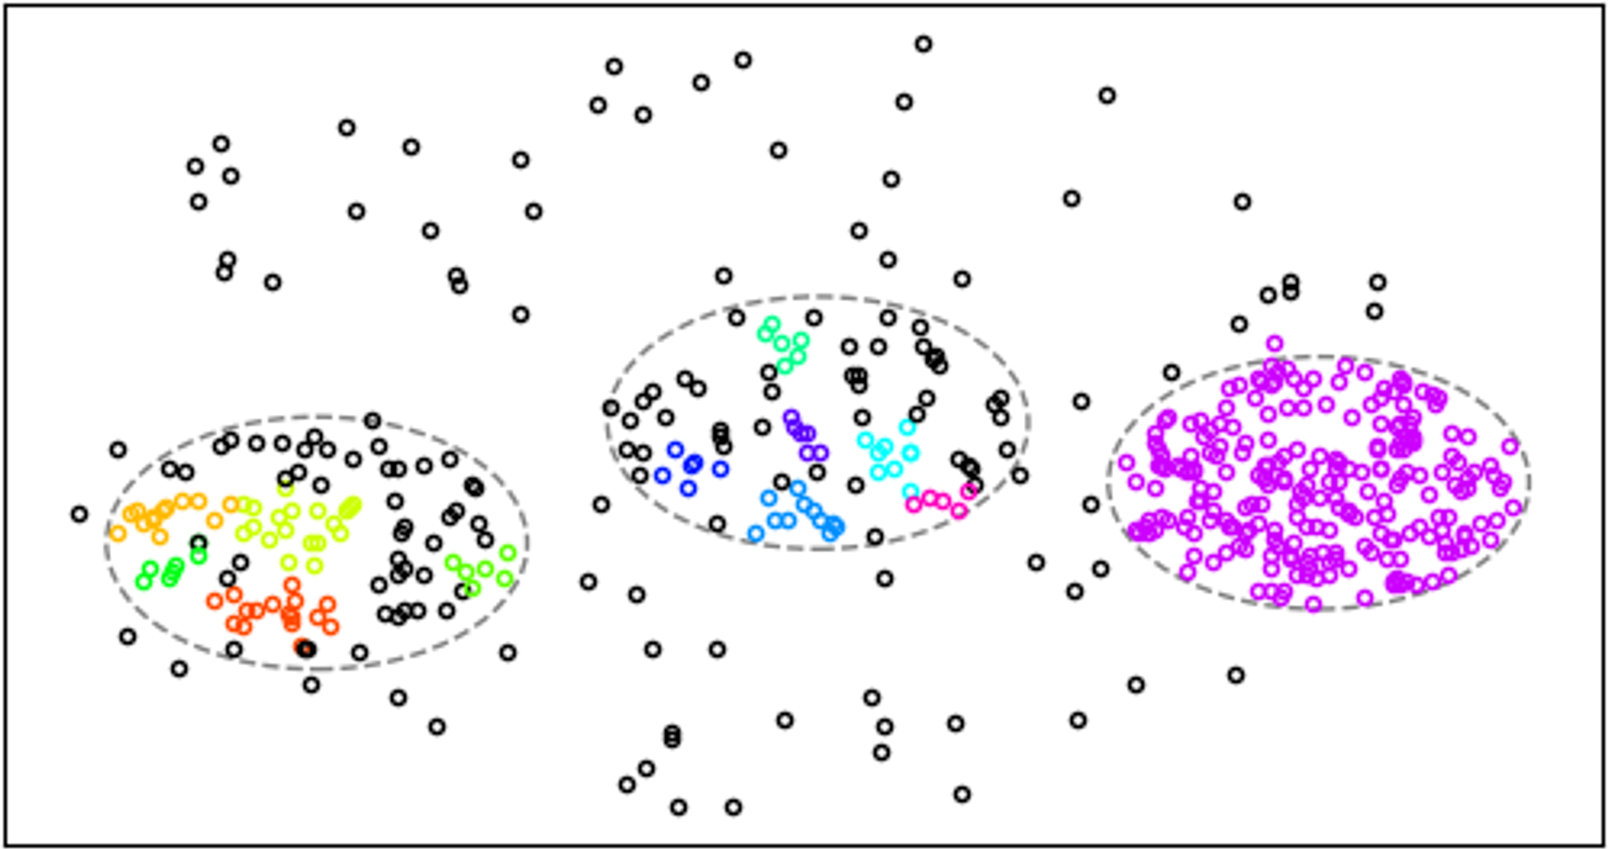
\includegraphics[width=\textwidth]{"Part 3 - Learning Systems/Unsupervised Learning/DBScan/figures/var-density.png"}
	\caption{An illustrative example is DBSCAN dealing with varying density 
	dataset. The colorful dots indicate the clusters identified by DBSCAN, 
	while the dash lines indicate the groundtruth clusters.}
      \label{fig:varying}
\end{figure}

However, DBSCAN may not be scalable to large datasets or 
high-dimensional dataset as it requires more memory and computing power. 
Recently, there is some debate on the runtime complexity of orginal DBSCAN in the
research community. The running time of DBSCAN depends on how many times the function
$RangeQuery(\cdot)$ is called. The original DBSCAN paper claims the average runtime 
complexity is 
$\mathit{\mathcal{O}(n \log n)}$. Gan et al. \cite{gan2015dbscan} argued that the algorithm actually requires $\mathcal{O}(n^{2})$.  However, their conclusion was questioned by other researchers. For example, Schubert et al. \cite{schubert2017dbscan} pointed out some inaccuracies in the way DBSCAN was represented by Gan et al. \cite{gan2015dbscan} instead of the algorithm itself, especially on the assumption about the performance of spatial index structures used to support the RegionQuery() method such as R-trees. Therefore, $\mathcal{O}(n^{2})$ is the worst case. Interested readers can dig more details by referrring to these 
research papers.  


Furthermore, for efficiency reasons, DBSCAN does not perform density estimation between 
all points. All neighbors within the $\epsilon$ radius of a core point are 
considered to be part of the same cluster as per defined direct density reachable.
If any of these neighbors is again a core point, transitively 
their density reachable neighbors are included. Non-core 
points in this set, or,
border points, are included as well as per density connectivity. 
Points which are not density reachable from
any core point are considered noise and do not belong to any cluster. However, 
if the density of the sample set is not uniform, DBSCAN performs poorly as illustrated in Figure \ref{fig:varying}. 

\section{Excercises}

\begin{enumerate}

\item Compared with K-means, what are the advantages and disadvantages of DBSCAN. 

\item Run the code provided by varying $MinPts$ and $\epsilon$ of the given example in this chapter to observe the impact of performance

\item Apply $k$-distance plot to find optimal $\epsilon$. You can use the SUN RGB-D dataset in this chapter. The code of solution can be found here \footnote{\url{https://gist.github.com/LinaYao/00f3b2cf65600f7b03df020c81cc5de9}}


\end{enumerate}

\bibliographystyle{unsrt}
\bibliography{bibliography}
